\documentclass[../ala_hataile.tex]{subfiles}
\begin{document}
\clearpage

\includepdf[pages=20-21, pagecommand={}]{sisasivut_19062018.pdf}

\includepdf[pages=24-27, pagecommand={}]{sisasivut_19062018.pdf}
	\twocolumn[\section{Mikä matemaattisissa tieteissä viehättää?} {\small {\itshape ``The most vitally characteristic fact about mathematics is, in my opinion, its quite peculiar relationship to the natural sciences, or more generally, to any science which interprets experience on a higher than purely descriptive level.''} --John V.\,Neumann}\vspace{0.5cm}]
	Kauneus on katsojan silmissä. Haluatko
	osata päätellä meteoriitin kolmi\-ulotteisen
	muodon sen varjo\-kuvien perusteella? Haluatko
	ymmärtää, miksi Maa\-pallolla on aina
	olemassa piste, jossa sekä paine että lämpö\-tila
	ovat täsmälleen samat kuin Maa\-pallon
	vastakkaisella puolella vastaavassa pisteessä?
	Miksi toiset äänestys\-järjestelmät ovat
	parempia kuin toiset? Haluatko ymmärtää
	miksi röntgenkuvalla on mahdollista saada
	käden poikkileikkauksen kuva? Miksi
	toisia ongelmia on mahdotonta ratkaista
	tietokoneella, kun taas toisia mahdollista?
	Voiko ongelmat laittaa vaativuusjärjestykseen?
	Haluatko ymmärtää miksi jotkut stereopiuhoihin
	tulleet solmut avautuvat itsestään
	ja toisia pitää avata vaivalla? Tiesitkö,
	että äärettömyyksiä on erikokoisia? Tiesitkö,
	että on olemassa joukko aksioomia,
	joista voi johtaa (melkein) koko matematiikan,
	vaikka tiedetään, että tällainen joukko
	ei koskaan voi olla täydellinen? Miten voidaan ennustaa,
	mitä tuotteita ostetaan vuoden päästä tai mikä nettisivu
	on suosituin? Miksi jokin lääketieteellinen koe 
	on parempi kuin toinen mittaamaan sairautta?
	
	Matematiikasta saattaa koulussa saada
	sellaisen kuvan, että se on laskemista, ei
	ymmärtämistä. Matemaattisiin tieteisiin siirryttäessä
	mielikuva jää elämään, vaikka laskeminen on vain pieni osa
	matematiikkaa, ja todellisuudessa asiantuntijat
	eivät juuri laske, vaan pikemminkin keksivät uusia
	laskutapoja ja menetelmiä ja mittavat niiden
	tehokkuutta, eikä silloin kysymys ole usein ollenkaan
	luvuilla pelailemisesta, kuten
	yllä olevista esimerkeistä voi nähdä. Koetus
	voikin olla hankala yliopistoon
	siirryttäessä. Eteen tulee paljon
	enemmän todistuksia ja menetelmiä kuin
	laskuja ja kaavoja.
	\begin{figure}[!b]
		\centering
		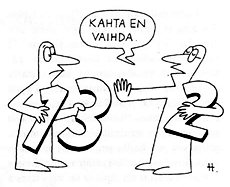
\includegraphics[width=0.5\textwidth]{kahtaen.png}
	\end{figure}
	\begin{figure*}[!b]
		\centering
		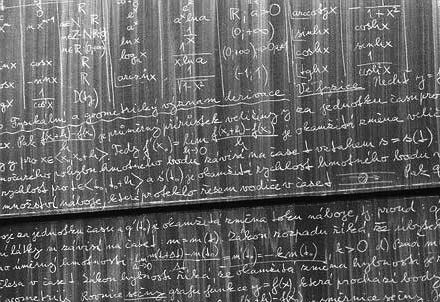
\includegraphics[width=\textwidth]{matikkataulu.png}
	\end{figure*}
	
	Keskeinen käsite on matemaattinen todistus.
	Todistuksen käsitteen oppiminen ja
	sisäistäminen on tärkein osa matematiikan
	opintojen alkuvaiheessa. Nyrkkisääntö: jos
	asia ei tunnu itsestään selvältä, et ole vielä
	ymmärtänyt sen todistusta. Todistus on siis
	tapa nähdä miksi jokin väite seuraa annetuista
	oletuksista. Ei enemmän eikä vähemmän.
	Joskus tuntuu, että väite on itsestään
	selvä jo valmiiksi, mutta onko itsestään selvää,
	että se seuraa annetuista oletuksista?
	Kannattaa kuvitella viereensä maailman
	skeptisin kaveri ja yrittää perustella hänelle
	väitettä.
	
	\begin{quote}
		``My brain is open.''\\-- Paul Erdös
	\end{quote}
	
	\vspace{0.5cm}
	\noindent\textsc{Vadim Kulikov}
	
	\twocolumn[\section{Matemaatikon paikka työelämässä} {\small {\itshape ``Matematiikan maisterin tutkintotodistus on merkki työnantajalle siitä, että henkilö on yrittänyt selviytyä jostain vaikeasta ja onnistunut siinä.''} --prof.\,Jouko Väänänen}\vspace{0.5cm}]
	Matematiikkaa tarvitaan kaikkialla, joten on vaikeaa antaa yksi\-selitteistä vastausta minne kaikkialle voi matemaattisten tieteiden kandi\-ohjelmasta päästä töihin. Paljon riippuu siitä, mihin on erikoistunut, ja minkä maisteri\-ohjelman valinnut. Ei kuitenkaan kannata liikaa stressata kurssien kanssa, koska paljon asioita oppii vasta työelämästä. Kandiohjelman yksi tärkeimmistä tehtävistä onkin tähän valmistaminen ja henkilö\-kohtaisen ajattelukyvyn kehittäminen. 
	\begin{figure}[h!]
		\centering
		
\includegraphics{partaproffa.png}
	\end{figure}

	Tutkijaksi jatkaminen on yksi vaihtoehto. Vaikka nyt saattaisikin tuntua siltä, että kaikki oleelliset matemaattiset tulokset olisi jo keksitty, ei näin kuitenkaan ole. Monet merkittävät kysymykset ovat yhä avoimia, minkä lisäksi matematiikassa kaivaudutaan yhä syvemmälle sekä kehitetään uusia teoriahaaraumia. Kumpula on kuuluisa erityisesti inversio-ongelmien tutkimisesta, mutta yleensä tohtoriopintojen jälkeen aloittelevan tutkijan tie vie ulkomailla sijaitsevaan yliopistoon. 
	
	Puhtaasti matematiikan tutkimisen lisäksi matematiikan taitajia tarvitaan myös muiden alojen tutkimusryhmiin. Esimerkiksi biologiassa on matemaattisen mallinnuksen avulla ymmärretty paremmin niin tautien leviämistä kuin lintujen käyttäytymistäkin. 
	
	Matemaattinen mallinnus ja kyky analysoida suuria data\-määriä herättävät kiinnostusta myös yritys\-maailmassa. Matemaattis\-painotteisen koulutuksen saaneita ihmisiä työskenteleekin niin puhelin\-operaattoreiden leivissä data-analyytikkoina kuin liikennöinti\-yrityksissä tavara\-kuljetuksien optimoijinakin.  
	
	Erilaisten ohjelmistojen tunteminen ja hallitseminen on usein tärkeää työelämässä, mutta ohjelmisto\-kehitys voi olla monen matemaattisista tieteistä valmistuneen opiskelijan päätyötä. Esimerkiksi monet kännykkä\-sovelluksia tai pilvi\-palveluita kehittävät yritykset tarvitsevat ohjelmoijia, joilla on vahva matematiikkatausta. Näin voi tapahtua esimerkiksi silloin, kun tarvitaan joku hiomaan ja kehittämään algoritmeja. Lisäksi kovaa matematiikkaa tarvitaan kone\-oppimisen ja parempien teko\-älyjen kehittämiseen. 
	
	Mainittakoon vielä lopuksi eräs pe\-rin\-tei\-sim\-mis\-tä yritys\-puolen työllistäjistä, pankki- ja vakuutus\-ala. Ensimmäisenä pankin työn\-tekijöistä tulee ehkä mieleen hymyilevä kassa\-virkailija, mutta jonkun on myös pystyttävä ennustamaan finanssi\-alan muutoksia, arvioimaan ihmisen elin\-ikää sekä tekemään malleja, joiden pohjalta annetaan yrityksille talous\-neuvontaa.
	
	\vspace{0.5cm}
	\noindent\textsc{Auli Salmi}
	
	\begin{figure*}[!b]
		\centering
		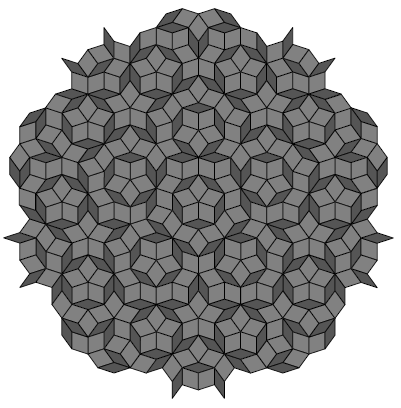
\includegraphics[width=0.7\textwidth]{geometrinen.png}
	\end{figure*}
	
	\begin{figure*}
		``Matematiikan ongelmat eivät lopu koskaan. Aiheet poikivat
		uusia ongelmia, eikä kaikkiin niihin löydy edes lopullista
		ratkaisua. Matematiikka elää huimaa kehityskautta,
		uusia työkaluja otetaan käyttöön kiivasta tahtia.''\\
		-- Professori Maarit Järvenpää
	\end{figure*}
	
	
	\twocolumn[\section{Matemaatikon sanasto} {\small {\itshape ``Muutamia termejä, joiden ymmärtäminen auttaa kummasti opiskelun alkumetreillä''}}\vspace{0.5cm}]
	\subsection*{Laskarit}
	Laskareista puhuttaessa tarkoitetaan
	joko laskuharjoitustehtäviä tai laskuharjoitusryhmiä.
	Kurssilla jaetaan yleensä 6~viikoittaista tehtävää, jotka opiskelijoiden
	tulee parhaansa mukaan ratkaista. Tämän
	jälkeen laskuharjoitukset katsotaan läpi
	laskariryhmissä, jolloin joku ryhmäläisistä
	pääsee esittelemään ratkaisunsa taululla.
	
	\begin{figure*}[!b]
		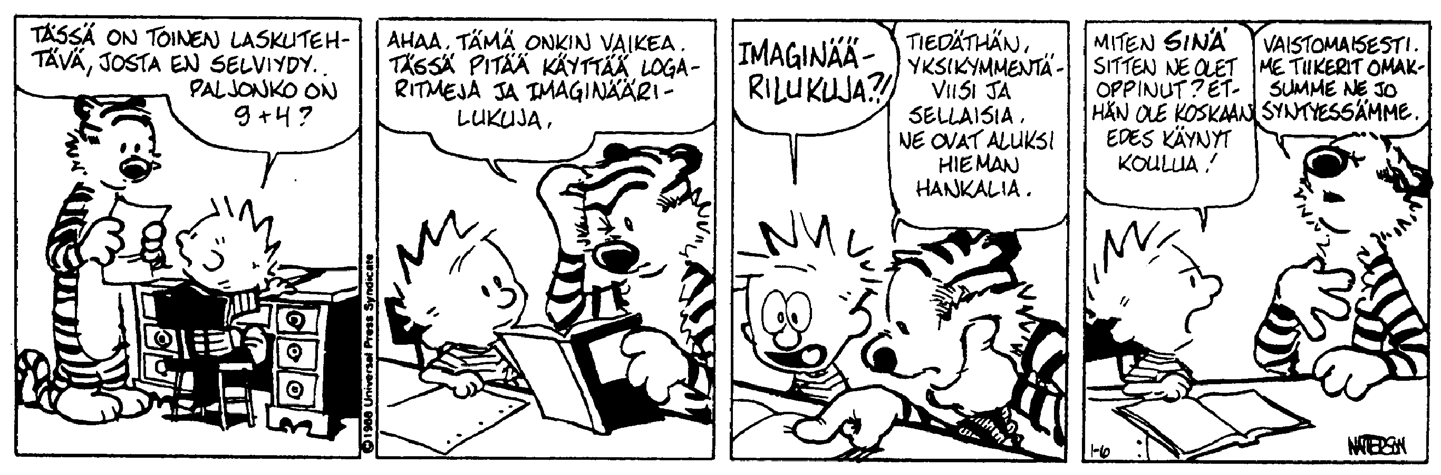
\includegraphics[width=\textwidth]{lassileevi_imaginaari.png}
	\end{figure*}
	Laskareiden pitäjä neuvoo ja opastaa -- hänestä
	kannattaakin ottaa kaikki hyöty irti.
	Jos omaan ryhmään ei jollain viikolla pääse,
	mahtuu jossain toisessa laskariryhmässä
	yleensä kyllä vierailemaan.
	\subsection*{Ohjaukset}
	Kursseilla Raja-arvot ja Differentiaalilaskenta (ja Sarjat?)
	laskuharjoitusryhmät
	on korvattu ohjausryhmillä.
	Tällöin osa laskuharjoitustehtävistä
	annetaan etukäteen ja tehdään ennen ohjausryhmän kaksituntista
	kokoontumista.
	
	Osa tehtävistä annetaan vasta kokoontumisen
	alussa ja ratkaistaan pienryhmissä
	kokoontumisen aikana. Myös etukäteen annetut
	tehtävät käydään läpi. Ohjausryhmät
	kokoontuvat kaksi kertaa viikossa.

	\subsection*{Kurssikoe}
	Suurimman osan kursseista voi suorittaa
	kurssikokeilla, joita on kurssista riippuen
	1--2~kappaletta periodien lopussa. Yleensä
	kurssikokeessa tehtäviä on neljä (joskus
	valitaan neljä tehtävää viidestä) ja niiden
	tekemiseen on yleensä aikaa kaksi tuntia.
	Yhdestä kurssikokeesta voi yleensä saada
	maksimissaan 24~pistettä ja kurssin lopuksi
	kaikkien kurssikokeiden pistemäärät lasketaan
	yhteen. Koepisteiden lisäksi lisätään
	kurssin aikana tehdyistä tehtävistä saatavat
	lisäpisteet.
	
	Läpi pääsee noin puolella pisteistä, mutta
	rajat vaihtelevat kursseittain. Jos koe sattuu
	olemaan jonkun toisen kurssin kokeen
	kanssa päällekkäin, ei kannata huolestua,
	sillä isoilla kursseilla järjestetään yleensä
	korvaava koe niille, jotka eivät päässeet
	paikalle varsinaisena koepäivänä.
	
	\subsection*{Yleistentti}
	Yleistentissä koealueena on koko kurssin
	sisältö, ellei olla luennoitsijan kanssa
	sovittu jotain muuta. Yleensä tehtäviä on
	viisi kappaletta ja niiden tekemiseen on aikaa
	neljä tuntia. Tentteihin ilmoittaudutaan
	netissä Web\-Oodissa (\url{www.helsinki.fi/weboodi})
	tai ottamalla kurssin vastuuhenkilöön
	yhteyttä (luennoitsija). Kesän aikana
	voi suorittaa kursseja kesätenteissä.
	\subsection*{Kurssi-ilmoittautumiset}
	Kursseille ilmoittaudutaan WebOodissa.
	Ilmoittautumisella ei sinänsä ole kiirettä,
	kaikki mahtuvat varmasti mukaan, tosin
	parhaat laskuharjoitusajat täyttyvät aika
	äkkiä.
	\subsection*{Ratkomo}
	Ratkomo eli sali C322 Exactumin kolmannessa kerroksessa 
	on oiva paikka laskea laskareita
	ja pohtia muuten vain matikkaa yksin tai
	yhdessä. Ratkomosta saa apua lähes kaikkiin
	matemaattisten tieteiden kursseihin.
	
	Ohjausluokan ohjaajat tunnistaa keltaisista
	huomioliiveistä, samalla tavalla kuin
	kisälliopetuskurssien ohjaajat. Ohjausta
	saa yleensä arkipäivisin klo 10--16 3.kerroksen
	käytävillä sekä Ratkomossa, joten muista
	katsoa myös kulman taakse liivien varalta.
	
	Kannattaa myös käyttää hyväkseen muita
	ahertavia opiskelijoita, he ovat voineet
	pohtia juuri samaa kysymystä kuin sinäkin.
	
	\subsection*{Arvostelu}
	Arvosteluasteikko on 0--5, nolla hylätty
	ja vain kokonaisluvut ovat käytössä.
	Arvosteluun vaikuttaa kurssista riippuen
	kurssikoemenestys, laskaritehtävien teko
	ja ohjauksissa käynti. Arvosanaa voi korottaa
	myös pyytämällä ylimääräisiä töitä, joita jotkut luennoitsijat mielellään antavat.
	\begin{figure}
		\centering
		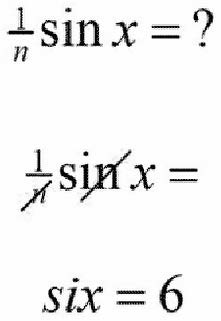
\includegraphics[width=0.5\columnwidth]{sin_six.png}
	\end{figure}
	
	Jos koet että sinua on
	kohdeltu kaltoin ja pisteet on laskettu väärin,
	käänny kokeentarkastajien ja kurssin
	luennoijan puoleen.

	\subsection*{Kisälliopetus}
	Jotkin ensimmäisen vuoden kurssit toteutetaan
	kisälliopetuksena, jolloin muita
	kursseja harvalukuisempien luentojen tukena
	on ympäri viikon auki oleva Ratkomo,
	johon voi mennä yhdessä tai yksin tekemään
	kurssin laskuharjoitustehtäviä.
	Paikalla on ohjaajia avustamassa tehtävien
	tekemisessä. Kursseissa tehtäviä on
	muita kursseja enemmän, mutta ne ovat
	pienempiä. Tehtävät myös palautetaan kirjallisena
	ja osa niistä tarkastetaan.
	Palautetuista tehtävistä saa pisteitä, jotka
	lisätään kokeista saatuihin pisteisiin.
	Tehtävien tekeminen siis todella kannattaa!
	
\subsection*{DIGest-menetelmä}
	
	DIGestive-menetelmässä opiskelijat palauttavat tekemänsä tehtävät Moodleen. Tehtävien tekemisen lisäksi oleellinen osa menetelmää on vertais\-arviointi. Joka viikko opiskelijalle arvotaan kahden anonyymin opiskelijan vastaukset, joiden palautus oli edeltävällä viikolla. Opiskelijalle annetaan malli\-vastaukset ja ohjeet, joiden avulla hän pisteyttää omat ja vertaisarvioitavat tehtävät. DIGest-menetelmän kursseilla yksi kolmas\-osaa kurssin pisteistä tulee harjoitus\-tehtävistä ja vertais\-arvionnista ja loput kaksi kolmas\-osaa kurssi\-kokeesta.
	
	\twocolumn[\section{Tärkeitä kursseja}]
	\subsection*{Perusopinnot}
	\subsubsection*{Johdatus yliopistomatematiikkaan (5~op)}
	Tämä perusopintoihin kuuluva kurssi
	on ehdottoman suositeltava suorittaa heti
	opintojen alussa.
	
	Kahden periodin mittaisen kurssin ensimmäisellä
	puoliskolla käydään läpi erilaisia
	joukkojen perusominaisuuksia ja niihin
	liittyviä käsitteitä ja tutustutaan erilaisiin
	joukkotodistuksiin. Lisäksi käydään läpi
	kompleksilukujen ominaisuuksia. Toisessa
	periodissa käydään läpi joukkojen alkioiden
	välisiä relaatioita ja kuvauksia sekä jatketaan
	kompleksilukujen läpikäyntiä.
	
	Kurssilla käytävät matemaattisen todistamisen
	menetelmät ovat tärkeimpiä
	seikkoja jotka tukevat matemaattista ymmärrystä
	tulevia kursseja varten. Kurssilla
	käytävistä asioista erityisesti relaatioista ja
	ekvivalenssiluokista on hyötyä Algebralliset rakenteet~I:n
	suorittamista varten.
	
	\vspace{0.5cm}
	\noindent\textsc{Jani Kaipainen}
	
	\subsubsection*{Lineaarialgebra ja matriisilaskenta~I+II (5+5~op)}
	Lineaarialgebran ja matriisilaskennan
	eli tuttavallisemmin ``liniksen'' kurssit johdattelevat
	opiskelijan matriisien, vektoreiden
	ja lineaarikuvausten maailmaan. Nämä
	kurssit kannattaa ehdottomasti suorittaa
	yhdellä kertaa, vaikka vain Linis-ykkönen kuuluu perusopintoihin. Kurssit keskittyvät yksi- ja
	useampiulotteisten vektoriavaruuksien peruskäsittelyyn.
	Mikä on vektoriavaruuden
	kanta? Miten matriiseja kerrotaan keskenään?
	Miten vektorien laskutoimitukset
	yleistetään mielivaltaisen moneen ulottuvuuteen?
	Näihin ja moneen muuhun kysymykseen
	saa kursseilla vastauksen.
	
	Homma pyörähtää käyntiin totuttelemalla
	vektorilaskentaan ja matriiseihin.
	Vektorit ovat eräs tapa puhua avaruuden
	pisteistä ja ne ovat tärkeä työkalu matematiikassa.
	Matriisit taas ovat eräänlaisia
	numerotaulukoita, joilla on omat laskutoimituksensa.
	Suuri paljastus ensimmäisellä
	kurssilla tuleekin, kun huomataan,
	että vektorit ovatkin oikeastaan eräänlaisia
	matriiseja. Matriiseja voi soveltaa monessa
	paikassa, kuten esimerkiksi yhtälöryhmien
	ratkaisussa, ja niiden avulla voidaan hahmottaa
	lineaarikuvausten toimintaa. Lineaarikuvaukset taas ovat erityisiä funktioita,
	joilla on monia miellyttäviä ominaisuuksia.
	Kurssi tarjoaa monia tärkeitä matemaattisia
	työkaluja ja kurssin keskeisten
	asioiden osaaminen takaa hyvän pohjan
	esimerkiksi Topologia I "-kurssille. Kurssit
	suoritetaan pitkälti pajaopetuksena, mikä
	tarkoittaa, että opiskelijan on syytä varautua
	lukemaan opintomonistetta itsekin,
	vaikka apua ja hyviä neuvoja on aina saatavilla
	pajaohjaajilta. Kurssit vaativat hieman
	työtä, mutta hyvin opitut asiat maksavat
	kyllä vaivan.
	
	\vspace{0.5cm}
	\noindent\textsc{Tuomas Salonen}
	
	\subsubsection*{Raja-arvot \& Differentiaalilaskenta (5~+~5~op)}
	Kursseilla käydään läpi periaatteessa
	lukiosta tuttuja käsitteitä, kuten lukujonojen
	raja-arvoja, funktioiden jatkuvuutta
	ja derivointia, mutta nyt matemaattisella
	tarkkuudella. Lukujonojen raja-arvon määritelmä
	tulee imeytymään selkärankaan, ja
	kurssin jälkeen jokainen ymmärtää miksi
	vanhemmat opiskelijat virnuilevat puhuessaan
	jostakin ``epsilonia pienemmästä''.
	
	Kursseilla suuressa osassa on myöskin
	totuttautuminen matemaattiseen ajatteluun.
	Lukiossa on varsin yleistä jättää tekemättä
	kaikki tehtävät, joissa tarvitsee todistaa
	jotain, mutta ensimmäisen yliopistosyksyn
	kuluessa asia tulee muuttumaan. Jatkuva
	todistaminen ja todistuksien taustalla
	olevan idean tajuaminen voi tuntua aluksi
	jännittävältä, mutta onneksi apua on paljon
	saatavilla. Kurssilla on käytössä
	viikoittaiset ohjaus\-ryhmä\-tapaamiset, joissa
	kokoonnutaan laskemaan ja tarkistamaan tehtäviä
	pienissä ryhmissä ohjaajan valvonnassa. Kannattaa
	myös yrittää tehdä kaikki tehtävät, vaikka et 
	ymmärtäisi aiheesta hölkäsen pöläystä,
	sillä pelkkä yrityskin riittää pisteiden saantiin
	ja ohjaaja kyllä selittää loput, elleivät kurssitoverit
	ehdi ensin.
	
	Luennoilla kannattaa ehdottomasti istua,
	sillä luentomateriaali kattaa vain kurssin
	virallisen matemaattisen osuuden, mutta
	luennoitsija saa luennoilla paukutettua päähän
	myös sitä, että miksi oikein olemme
	tekemässä tätä.
	
	\vspace{0.5cm}
	\noindent\textsc{Rami Luisto}
	
	\subsubsection*{Integraalilaskenta (5~op)}
	Kurssi Integraalilaskenta on suoraa jatkoa Raja-arvoille ja Differentiaali\-laskennalle. Kurssilla perehdytään siihen, miten perinteinen Riemannin integraali toimii, ja johdetaan lukiosta tutut integrointi\-kaavat.
	
	Edeltäjistään poiketen kurssilla käytetään Digest-menetelmää, jossa opiskelijat palauttavat vastauksensa sähköisesti ja pääsevät tarkastamaan muiden tehtäviä. Tehtävien palauttaminen on laskuharjoituksiin osallistumista työläämpää, mutta anonyymeistä tehtävistä saa henkilökohtaista palautetta ja pääsee myös näkemään miten muut ovat samaa tehtävää lähestyneet. 
	
	Nämä kolme kurssia liittyvät tiiviisti toisiinsa
	ja ne kannattaa suorittaa ensimmäisenä
	vuonna. Ne ovat osa perusopintoja
	mutta, mikä tärkeämpää, ne johdattavat
	tuoreen opiskelijan taidokkaasti matematiikan
	uuteen maailmaan.
	
	\vspace{0.5cm}
	\noindent\textsc{Auli Salmi}
	
	\begin{figure*}[!b]
		\centering
		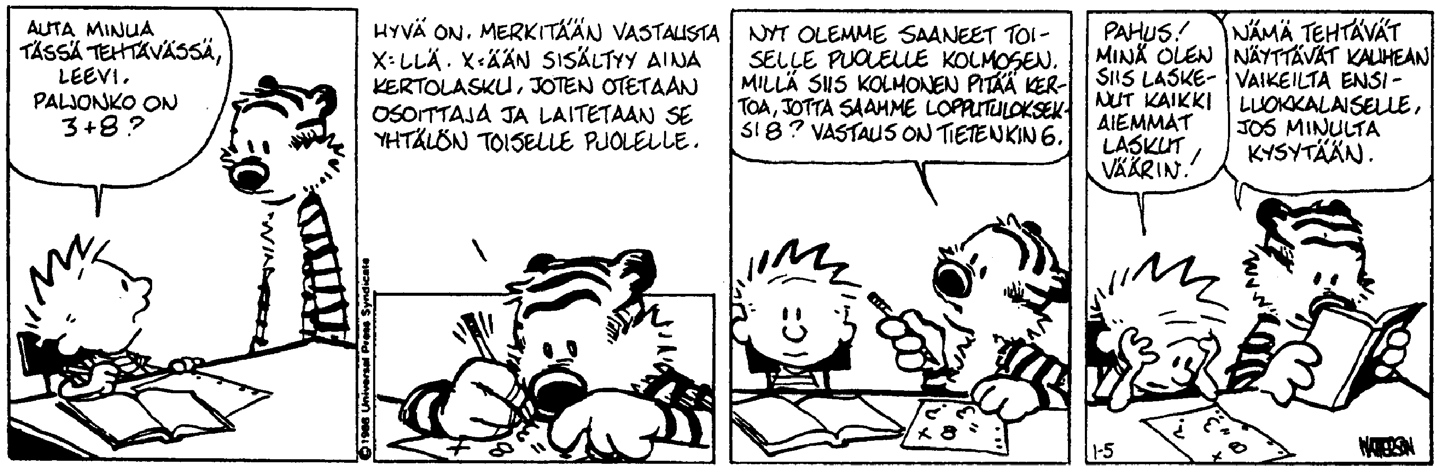
\includegraphics[width=\textwidth]{lassileevi_imaginaari2.png}
	\end{figure*}
	

	\subsection*{Aineopinnot}
	\subsubsection*{Sarjat (5~op)}
	Ensimmäisessä periodissa menevä Sarjat kannattaa ottaa heti toisen opiskeluvuoden syksynä. Kurssi käyttää samaa kirja kuin Raja-arvot, Differentiaalilaskenta ja Integraalilaskenta, minkä vuoksi se on hyvin saman tyylinen yllä mainittujen kurssien kanssa. Nimensä mukaisesti kurssilla tutustaan erilaisiin sarjoihin, esitellään työkaluja niiden suppenemisen tutkimiseen ja opetellaan, miten äärettömän suppenevan sarjan alkioita järjestelemällä voi kyseinen sarja saada minkä tahansa raja-arvon.
	
	\vspace{0.5cm}
	\noindent\textsc{Auli Salmi}
	\subsubsection*{Topologia IA+IB (5+5~op)}
	Kurssilla tutustutaan siihen, miten kursseilta Raja-arvot ja
	Differentiaali\-laskenta tutuksi tulleet jatkuvuus ja suppeneminen
	voitaisiin yleistää abstraktimpiin
	tilanteisiin. Tämä toteutetaan kurssilla
	määrittelemällä etäisyyden käsite hyvinkin
	mielivaltaisissa tilanteissa. Esimerkiksi
	New Yorkissa kahden pisteen välinen kävelymatka
	voi olla eri kuin suoraa pitkin
	mitattu etäisyys. Kurssilla ei ole nimellisiä
	esitietovaatimuksia, mutta niin sanotusta
	``matemaattisesta kypsyydestä'' on hyötyä.
	(Eli suomeksi syksyn kurssit ovat henkisesti
	tarpeen.)
	
	Kurssin asioita tulee tarvitsemaan jatkuvasti
	(heh) jatkossa. Moni vaativampi
	kurssi tarvitsee topologian tietoja esitietoinaan.
	Kursseilla Topologia~I ja II on oppimateriaalina
	samannimiset kirjat, jotka
	ovat suomenkielisten matematiikan kirjojen
	ehdotonta huippua.
	
	\vspace{0.5cm}
	\noindent\textsc{Rami Luisto}
	
	\subsubsection*{Johdatus logiikkaan I+II (5+5~op)}
	Logiikka I on syksyisin tarjottava kurssi
	ja useat käyvätkin sen ensimmäisen tai
	toisen opiskeluvuoden syksyllä. Kurssilla
	ei tosin ole mitään esi\-tieto\-vaatimuksia,
	joten sen voi käydä melkein missä tahansa
	vaiheessa opintojaan. Kurssilla tutustutaan
	propositio- ja predikaatti\-logiikan alkeisiin,
	päättelyyn ja semanttisiin puihin. Kurssista on keväisin tarjolla myös
	englanninkielinen verkkokurssi, jos syksyllä ei kalenteri anna periksi.
	Ensimmäinen on vaikeustasoltaan varsin mukava,
	mutta on annettava pieni varoituksen
	sana toisesta. Logiikka~I:llä
	käsitellään propositio\-logiikkaa, ja siinä tapahtuvia
	päättelyitä ynnä muita. Tämä on
	vielä varsin mekaanista toimintaa, mutta
	Logiikka II:ssa siirryttäessä
	predikaatti\-logiikkaan muuttuvat päättelyt
	haastavammiksi. Ei siis kannata tuudittautua
	ensimmäisellä kurssilla uneen vaikka
	asiat tuntuisivat helpoilta, sillä asiat muuttuvat
	salakavalasti haastavammiksi seuraavalla kurssilla.
	
	Seuraavan kosketuksen logiikkaan saa esimerkiksi
	kurssilta Matemaattinen logiikka.
	
	\vspace{0.5cm}
	\noindent\textsc{Rami Luisto}
	
	\subsubsection*{Differentiaaliyhtälöt I+II (5+5~op)}
	Kuinka kauan kestää jääpallon sulaminen?
	Mitä rataa pitkin juoksee susi, kun
	yrittää saada paraabelia pitkin juoksevaa
	jänistä kiinni? Miten taudit etenevät populaatioissa?
	Tämän tyyppiset kysymykset
	ovat motivaationa differentiaaliyhtälöiden
	tutkimukselle.
	
	Näillä kursseilla tutustutaan differentiaaliyhtälöiden
	perusteisiin -- opetellaan
	ratkaisemaan tiettyjä yksinkertaista muotoa
	olevia differentiaaliyhtälöitä ja tunnistamaan
	milloin nämä yhtälöt ovat yksinkertaista
	muotoa.
	
	Ensimmäisessä osassa käsitellään lineaarisia
	ja homogeenisia differentiaaliyhtälöitä.
	Toisessa osassa käydään differentiaaliyhtälöiden
	yleistä teoriaa ja yhtälösysteemejä;
	tässä vaiheessa olisi hyvä jo osata
	osittaisderivoinnin lisäksi vähän lineaarialgebraa
	ja täsmällisen analyysin alkeitakin.
	Kurssi sopii hyvin 2.\,opiskeluvuoden kevääseen
	Vektorianalyysin rinnalle, tällöin
	esitiedotkin ovat varmasti kunnossa. Kurssia
	ovat viime aikoina pitäneet innostavat
	luennoitsijat, ja oppimateriaalina käytetty
	Petri Olan monistekin on varsin hyvä.
	
	\vspace{0.5cm}
	\noindent\textsc{Vadim Kulikov}
	
	\subsubsection*{Mitta ja integraali (5~op)}
	Pituus, pinta-ala ja tilavuus ovat meille
	pienestä tuttuja käsitteitä: nämä ovat esimerkkejä
	mitoista. Intuitiivisesti haluamme,
	että jokaiseen joukkoon (esim. tason
	osajoukkoon) liittyy luku, joka kertoo sen
	mitan (pinta-alan). Haluamme kenties, että
	kun joukkoa siirretään vähän sivulle, mutta
	pidetään saman muotoisena ja "-kokoisena,
	sen mitta pysyisi muuttumattomana vaikka
	siitä tuleekin toinen tason osajoukko. Haluamme,
	että jos joukko $A$ sisältyy joukkoon
	$B$, niin $B$:n mitta olisi vähintään $A$:n mitta.
	Kurssilla esitellään eräs tapa konstruoida
	mitta Euklidiseen avaruuteen, jonka erikoistapauksia
	pituus, pinta-ala ja tilavuus
	ovat. Valitettavasti kaikkia yllä mainittuja
	ehtoja ei voi noudattaa yhtä aikaa. Se mistä
	luovutaan on ensimmäinen: kaikkiin joukkoihin
	ei saada liitettyä lukua. Tällaisia
	joukkoja kutsutaan epämitallisiksi -- niitä
	ei voi mitata.
	
	Sittemmin kurssilla määritellään Lebesguen
	integraali, todistetaan, että se on monessa
	suhteessa parempi kuin Riemannin
	integraali. Muun muassa Riemannin integraali
	käyttää suhteellisen spesifisiä reaalilukujen
	ominaisuuksia, mutta Lebesguen integraali
	voidaan määritellä missä tahansa,
	missä on (jokin) mitta.
	
	Kurssi on vain yhden periodin mittainen,
	mutta haastava. Laskuharjoituksia
	kannattaa tehdä ahkerasti.
	
	\vspace{0.5cm}
	\noindent\textsc{Vadim Kulikov}
	\subsubsection*{Vektorianalyysi I+II (5+5~op)}
	Entä jos funktiot menevätkin 3-ulotteisesta
	avaruudesta 2-ulotteiseen? Entä
	jos $n$-ulotteisesta $m$-ulotteiseen? Hiukkasen
	liike\-rataa avaruudessa kuvaa funktio 1-ulotteisesta avaruudesta 3-ulotteiseen.
	
	Saippuakuplaa kuvaa pinnan (2-ulotteisen
	avaruuden) upotus (jatkuva bijektio)
	3-ulotteiseen. Missä tällainen funktio saavuttaa
	maksiminsa? Mitä tarkoittaa tällaisen
	funktion derivaatta?
	\begin{figure}[!b]
		\centering
		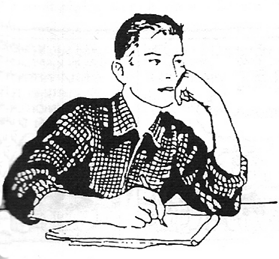
\includegraphics[width=\columnwidth]{pohtiva.png}
	\end{figure}
	
	Vektorianalyysi on ainakin alkuviikoilla
	melko suoraa yleistystä Differentiaalilaskennan
	jatkuvuus- ja derivaattaopista useampiulotteiseen
	tapaukseen. Tämä on kenties yksi
	syy, miksi todistuksien yksityiskohtia ei
	käydä kovin tarkasti: uskotaan, että opiskelija
	osaavat täydentää itse puuttuvat kohdat.
	Historiallisesti vektorianalyysi on syntynyt
	Newtonin mekaniikasta. Planeettojen
	liikeradat, rakettien tarvitsema energia gravitaatio-
	tai magneettikentässä, nesteiden
	ja kaasujen virtaukset sekä painejakaumat
	ovat esimerkkejä luonnollisista vektorianalyysin
	sovelluksista.
	
	Kurssi kuuluu ehdottomasti matemaatikon
	yleissivistykseen ja on välttämätön soveltavaan
	matematiikkaan, matemaattiseen
	fysiikkaan ja tilastotieteeseen suuntaville.
	
	\vspace{0.5cm}
	\noindent\textsc{Vadim Kulikov}
	
	\subsubsection*{Algebralliset rakenteet~I+II (5+5~op)}
	Kaikki tietävät, miten yhteen- ja kertolasku
	toimivat. Kuitenkin voidaan kysyä,
	miksi ne toimivat juuri näin. Voisivatko ne
	kenties toimia jotenkin muuten? Voiko olla
	muunlaisia laskutoimituksia? Algebralliset
	rakenteet asettaa tämän luonteiset kysymykset
	opiskelijan eteen kenties ensimmäistä
	kertaa. Kursseilla opiskelija joutuu
	taivuttamaan ajatuksiaan hyvin yleiselle
	tasolle. Kysymys on asioista, jotka porautuvat
	luvuilla laskemisen ytimeen.
	
	Kurssit alkavat käymällä nopeasti läpi
	perusasiat joukoista, kuvauksista ja relaatioista
	ja etenee sitten vauhdikkaasti
	erilaisiin algebrallisiin rakenteisiin. Opiskelijalle
	tulee tutuksi, miten määritellään
	laskutoimitus ja milloin joukosta, jonka
	alkioille laskutoimitus on määritelty, tulee
	ryhmä. Käy ilmi, että tuntemamme laskusäännöt
	ja luvut ovat vain erikoistapauksia.
	Kurssin erikoisimpiin ja kiehtovimpiin asioihin
	kuulunevat sykliset ryhmät, ekvivalenssiluokat
	ja "-relaatiot ja lopussa kaiken
	kruunaa ryhmien homomorfialause.
	
	Tarjolla on siis tiukka paketti työkaluja
	ja uusia näkökulmia matematiikan maailmaan.
	Kurssi vaatii hieman aivojen nyrjäyttelyä,
	mutta avarakatseinen opiskelija
	saa kyllä palkkionsa, kun huomaa oppineensa
	voimakkaita työkaluja monimutkaistenkin
	ongelmien ratkontaan. Kyseessä
	on pajakurssi, joten siihen sisältyy paljon
	omatoimista oppikirjan lukemista ja kunnon annos tehtäviä. Apua on kuitenkin tarjolla
	riittämiin kysymällä pajaohjaajilta, ja
	matematiikasta pitävälle kurssin aiheiden
	silkka mielenkiintoisuus pitää motivaatiota
	yllä.
	
	Algebralliset rakenteet~I \& II ovat perustavanlaatuisia
	kursseja, joka on syytä
	käydä mahdollisimman pian. Sen sisältämät
	asiat ovat osa matemaattista perussivistystä
	ja niiden hallitseminen helpottaa
	tulevien asioiden omaksumista. Etukäteen
	on hyvä olla takataskussa tiedot kursseista
	Lineaarialgebra ja matriisilaskenta~I \& II
	sekä kurssista Johdatus yliopistomatematiikkaan.
	
	\subfile{sections/tilastotiede}
	
	\begin{figure*}[!b]
		Muista myös Matrixin ja Moodin tarjoamat kurssikuvaukset ja opinto-oppaat!\\ \url{https://wiki.helsinki.fi/display/Matrix/Kurssikuvauksia}\\
		\url{https://wiki.helsinki.fi/display/moodi/Moodin+varjo-opinto-opas}
	\end{figure*}
\end{document}